\section{Introduction}\label{sec:intro}

\paragraph{Motivation.} Automated fiber placement and continuous-fiber printing lay
composite tows along curved paths, so the local fiber orientation $\theta(\bm x)$ of a
part becomes a design field. That field is routinely designed for \emph{static}
performance: stiffness and strength under a minimum turning-radius constraint, with the
toolpath carried through the optimization \cite{wong2025}. A carbon/epoxy lamina is
also strongly \emph{acoustically} anisotropic. Its quasi-longitudinal wave speed
differs by a factor of almost four between the fiber and transverse directions. This
raises the possibility that the same manufacturing freedom, with no change of material
or mass, could steer in-plane elastic waves: concentrate vibration where it is wanted,
keep it from where it is not, or hide an obstacle from it.

\subsection{Related work and positioning}\label{sec:related}
\paragraph{Fiber-orientation design.} Curvilinear fiber formats were introduced to raise
buckling loads and relieve stress concentrations \cite{hyer1991}. Variable-stiffness
laminates are now designed routinely for stiffness and buckling \cite{gurdal}. Orientation
is also optimized element-wise in discrete-material and continuous-orientation topology
optimization \cite{stegmann2005,nomura2015}. Continuous-fiber additive manufacturing
\cite{matsuzaki2016} has made arbitrary in-plane fiber fields buildable. Wong et al.\
integrated toolpath generation and a local fiber-curvature limit into
compliance-minimizing topology optimization \cite{wong2025}. We adopt their CS-RBF
orientation field and curvature constraint. Smoothness and manufacturability of optimized orientation fields are active topics in their own
right: smooth-orientation filters in anisotropic topology optimization \cite{jiang2024}, segmentation
of an optimal stiffness field into manufacturable curvilinear patches \cite{sheikhi2024}, and models
of the gaps and overlaps of tow placement \cite{fayazbakhsh2013,pagani2025}. Curvature-constrained
orientation design is therefore not new, and we do not claim it. This work, like most of the
literature, targets \emph{static}, \emph{modal} or forced-vibration objectives: the fundamental
frequency \cite{abdalla2007,pagani2025}, the natural modes of curvilinear-fiber laminates
\cite{akhavan2011}, and minimum sound radiation from vibrating laminates by discrete orientation
selection \cite{niu2010}. Anisotropic composite layouts have also
been designed to shield, focus and cloak \emph{diffusive} heat flux
\cite{dede2013smo,dede2013apl}. Lu and Tong optimized macrostructure, microstructure and spatially varying orientation of
anisotropic material concurrently for mechanical cloaking \cite{lutong2025}, and Olsson and Wall chose
fiber directions for exact partial cloaking in the inextensible limit \cite{olsson2011}. Our problem
differs from these in three ways: the field is time-harmonic in-plane elastodynamics, the
orientation of one fixed lamina is the \emph{only} design field (no density, topology or material
change), and the field must respect the tow-curvature limit. A targeted search found no prior work
that optimizes fiber orientation alone under that limit to steer elastic waves; the search was not
exhaustive.

\paragraph{Wave control by graded media.} Transformation optics \cite{pendry2006} and
transformation elastodynamics \cite{milton2006,norris2008,brun2009,norrisshuvalov2011} prescribe material
fields that bend waves arbitrarily. The required media are singular at the inner
surface of a cloak. With isotropic stiffness the density must become infinite there, and a
finite-mass cloak needs anisotropic (pentamode) stiffness instead \cite{norris2008}; for
in-plane elasticity the transform keeps the Navier form but with a tensor that is singular
at the inner boundary and lacks the minor symmetries of a Cauchy solid
\cite{brun2009,norrisshuvalov2011}, and in general the transformed equations are not of
Cauchy-elastic form \cite{milton2006}, so no lamina can realize them. Pre-stressing a
hyperelastic solid is another route to the required properties
\cite{parnell2012,norrisparnell2012}. Olsson and Wall showed that inextensible
fibers in a variable direction give form-invariant equations of motion and exact partial
cloaking at all frequencies \cite{olsson2011}; this is the idealized limit of unbounded
anisotropy, which a real lamina does not reach. Ground-plane (carpet) cloaks, which only
need to mimic a flat reflecting surface, can be broadband with bounded (natural or layered) anisotropy
\cite{chen2011,popa2011}. In practice, elastic lenses and wave guides
use graded index fields made from thickness variations \cite{climente2014} or
phononic crystals \cite{tol2017}, mostly for flexural waves in isotropic plates. Adjoint
inverse design of plate wave devices has used pinning, mass loading and grading
\cite{capers2023}. Topology optimization of wave problems is well developed for band
gaps, acoustics and photonics \cite{sigmund2003,duhring2008,jensen2011}, including
low-contrast optical cloaks \cite{andkjaer2011} and acoustic cloaks \cite{andkjaer2013}, and the
single-frequency optima it produces are known to be narrowband, which motivates
band-averaged objectives \cite{jensen2005,andkjaer2013}. In these approaches the design variable is the
\emph{amount} of material or its local stiffness, not its \emph{orientation}.

\paragraph{Waves in anisotropic plates.} In anisotropic solids, energy does not travel
along the wave normal: the group velocity is skewed toward stiff directions
\cite{auld,rose2014}. In fiber-reinforced composite plates this focuses guided waves into the directions of
minimum slowness, which are the stiff directions \cite{chapuis2010}. In some anisotropic plates the power flux of slow guided waves can even
be perpendicular to the wave vector \cite{kiefer2023}. In non-destructive evaluation the skew
is a nuisance to be compensated. Here it is the mechanism to be designed.

\paragraph{What is new here.} The ingredients are known: group-velocity skew in anisotropic solids
\cite{auld,chapuis2010}, inverse design of wave devices \cite{sigmund2003,capers2023}, and
curvature-constrained orientation fields \cite{wong2025}. The contribution is their combination for a
\emph{wave-control target} with orientation as the only design field, and an analysis of
\emph{energy transport} that separates what the fibers do from what the finite plate does.
Specifically: (i) the mechanism, energy channeling by group-velocity skew, is tested prediction by
prediction, including against a ray prediction computed from the fiber field alone and against
fields that were never optimized; (ii) an exact identity splits every focus gain into redirection and
resonant whole-field growth, and the redirection is cross-checked against the share of injected power
the target absorbs; (iii) following band-objective practice \cite{jensen2005,andkjaer2013}, every design
is evaluated across a band and against a series of absorbing layers. We show that orientation is a
distinct design channel for wave control; we do not compare it with thickness grading, material
redistribution or multi-ply layouts, and do not claim it is superior to them. The orientation fields satisfy
the tow-curvature limit pointwise; we call them \emph{tow-curvature-constrained} rather than
manufacturable, because tow width, coverage and defects are only estimated (Sec.~\ref{sec:asbuilt}).

\subsection{Question, hypothesis and predictions}\label{sec:qh}
\paragraph{Scientific question.}
\begin{quote}\itshape
How much control over an in-plane elastic wave field can the fiber orientation of a
continuous-fiber composite exert, at fixed material and mass and under the tow-curvature
limit of automated placement? By what mechanism does that control act, and what bounds
it?
\end{quote}

\begin{figure}[!tbp]
\centering
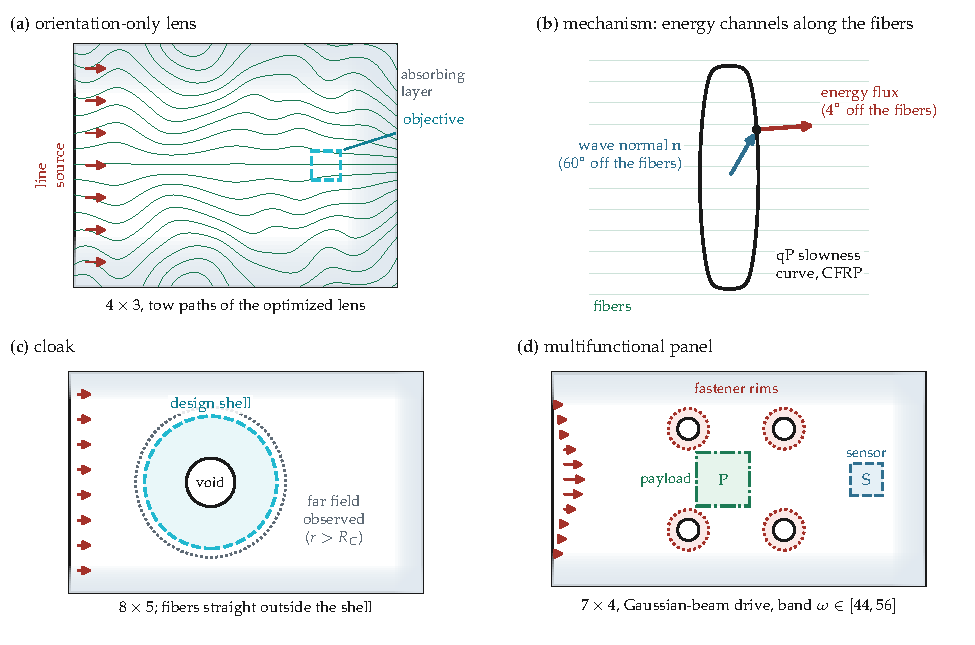
\includegraphics[width=\textwidth]{figs/wt_schematic.pdf}
\caption{The three problems and the mechanism. \textbf{(a)}~The lens: a $4\times3$ CFRP plate
driven by an $x$-directed line source at its left edge, with absorbing layers on the other three
edges (shaded), the tow paths of the optimized lens, and the objective region (dashed).
\textbf{(b)}~Why fibers channel energy: the quasi-P slowness curve of the CFRP lamina (fibers
along $x$). The energy of a plane wave travels along the outward normal to this curve, so a
wave whose normal is $60^\circ$ off the fibers carries its energy only a few degrees off them
(Sec.~\ref{sec:theory}). \textbf{(c)}~The cloak: a traction-free void cut from the mesh, the
design shell in which the orientation may change (dashed), and the far-field observation
region beyond $R_C$ (dotted). \textbf{(d)}~The multifunctional panel: four fastener holes with
their rim regions (dotted), the payload P and sensor S, and a Gaussian-beam drive.}
\label{fig:schematic}
\end{figure}

\paragraph{Hypothesis.} (Fig.~\ref{fig:schematic}.) In a strongly anisotropic lamina, the energy of a plane wave does
not travel along its wave normal. It is skewed toward the fiber direction, by up to
$\WSkewMax^\circ$ for CFRP (Sec.~\ref{sec:theory}). Most wave normals therefore carry their
energy within a narrow cone about the fibers. We hypothesize that a fiber field acts as a
field of \emph{energy streamlines}: designing $\theta(\bm x)$ designs where vibration
energy goes, because energy is channeled along the fibers. The hypothesis has stated conditions. It
concerns the qP part of the field. It is a ray (WKB) statement, so it requires the fibers to turn
slowly on the scale of the wavelength. And it ignores reflections and interference. Where these
conditions fail (long wavelengths, sharply turning fibers, standing-wave nodes, boundaries) we expect
channeling to fail, and we measure where it does. Section~\ref{sec:theory}
makes this precise. It predicts:
\begin{enumerate}[label=\textbf{W\arabic*},leftmargin=2.4em,itemsep=1pt]
\item An isotropic plate offers no orientation control at all.
\item The robust effect of an optimized field is \emph{redirection}: a larger share of
  the wave energy, and of the injected power, in the target. Because the energy skew of a homogeneous
  lamina does not depend on frequency, redirection should be broadband over the wavelengths for which
  the ray picture holds. Any gain beyond redirection that appears at the design frequency is
  whole-field build-up, consistent with resonance, and narrowband.
\item In the optimized designs, the local energy flux follows the fiber direction where the
  fibers turn slowly, and a ray prediction from the fiber field alone reproduces the redirection.
\item Redirection grows with the lamina anisotropy, tracking the share of wave normals
  that the lamina channels toward its fibers.
\item Energy can follow a curving fiber field only as fast as the field may turn, so the
  tow-curvature limit bounds the redirection. Canceling the field of a finite scatterer in free space (a full cloak, not a
  ground-plane cloak) needs the singular anisotropy of transformation media. With the
  bounded anisotropy of a real lamina it must rely on interference, and we predict it to be
  narrowband.
\end{enumerate}

\subsection{Approach and findings}
\paragraph{Approach.} We solve the genuine two-dimensional orthotropic time-harmonic
problem: the rotated plane-stress stiffness $\bm D_f(\theta)$ with
$E_{f1}/E_{f2}=14.6$, light structural damping, and an absorbing sponge. A real
four-field split runs it on a real-arithmetic \texttt{PETSc}/\texttt{dolfinx} build,
and automatic discrete adjoints give the orientation sensitivity. The field is
parametrized by smooth compactly supported radial basis functions and bounded by the
tow curvature. We optimize a lens and a cloak, then test each prediction by
decomposing the gains, sweeping frequency, measuring the energy-flux field, varying the
anisotropy, and tightening the curvature limit, each with multiple optimizer starts where the result depends on
them. A band-averaged multifunctional panel shows how the results translate into a design practice.

\paragraph{Organization.} Section~\ref{sec:model} states the model and its physical scales,
Sec.~\ref{sec:theory} the channeling theory and the ray prediction, Secs.~\ref{sec:fem}--\ref{sec:adj}
the discretization, adjoint and orientation parametrization, Sec.~\ref{sec:results} the tests of
W1--W5, the as-built check and the multifunctional panel, and Sec.~\ref{sec:discussion} what is and is
not established.
